\section{Results}
\label{sec:results_ukb_assoc}

\subsection{Phenotype Correlations}
\label{sub:phenotype_correlations}

Phenotypical correlations are displayed in Figure~\ref{fig:corr_pheno}. 
As expected the data contains considerable correlations between happiness and neuroticism.Further, strong correlations are also present between aggresion and impulsive aggression.
In contrast correlations between risk taking as well as IQ with other analysed phenotypes is low.
All correlations were significant at $p\leq 0.05$ after adjusting for multiple testing  with Bonferroni correction.

\begin{figure}[htpb]
  \centering
  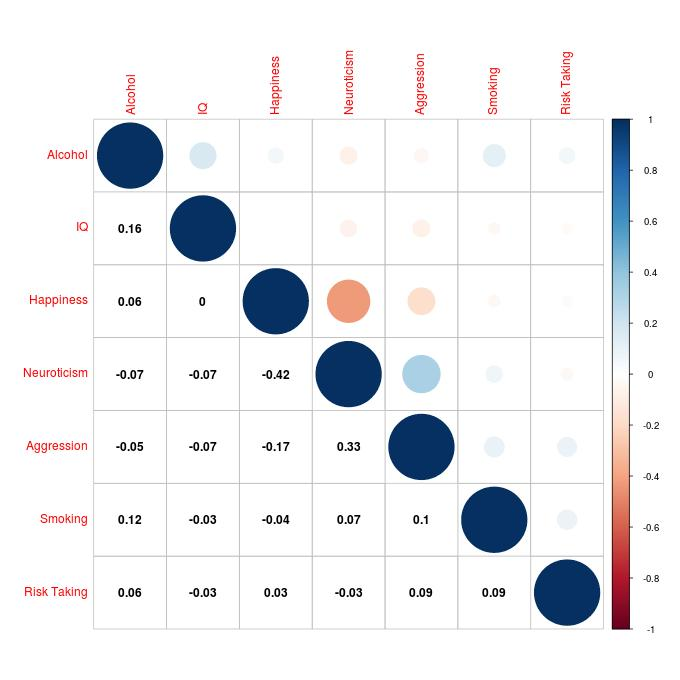
\includegraphics[width=0.8\linewidth]{ukb_assoc/figure/phenotype/corr_plot_circle_full.jpeg}
  \caption{Phenotypical correlations among analysed phenotypes}\label{fig:corr_pheno}
\end{figure}


\subsection{Impulsive Aggression}
\label{sub:impulsive_aggression_gwas}

No significant hits were identified in $\sim37,320$ subjects (see Figure~\ref{fig:gwas_impAgg}).  This is unfortunate but not surprising giving the low number of individuals.  Further no population stratification has been identified and SNP heritability is relatively low.
Table~\ref{tab:LDscImpAgg} shows both intercept and rato of LD-score regression, as well as $\lambda_{GC}$ and estimated SNP heritability.
Observed heritability is with $5.32\%$ relatively low.
Both $\lambda_{GC}$ and intercept are close to $1$ suggesting no population stratification. 
Further, the ratio estiamte, which is a measure of the propotion the LD-score intercepts ascribes to factors other than polygencity is between the acceptable range of 10\%--20\%.


\begin{figure}[!htpb]
  \begin{subfigure}[t]{.5\textwidth}
    \centering
    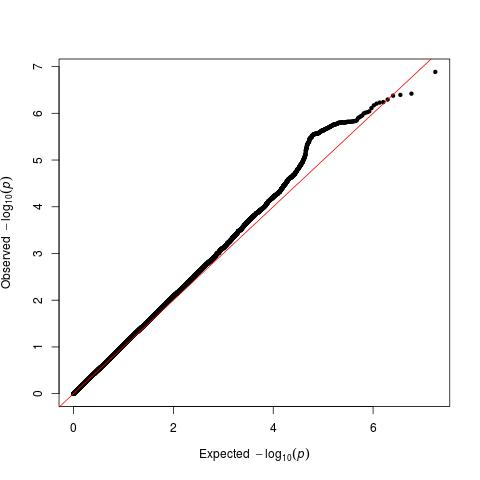
\includegraphics[width=0.8\linewidth]{{ukb_assoc/figure/qq_plots/qq_plot_4526}.jpeg}
    \caption{QQ-plot for Impulsive aggression}\label{fig:ImpAgqq}
  \end{subfigure}
  \begin{subfigure}[t]{.5\textwidth}
    \centering
    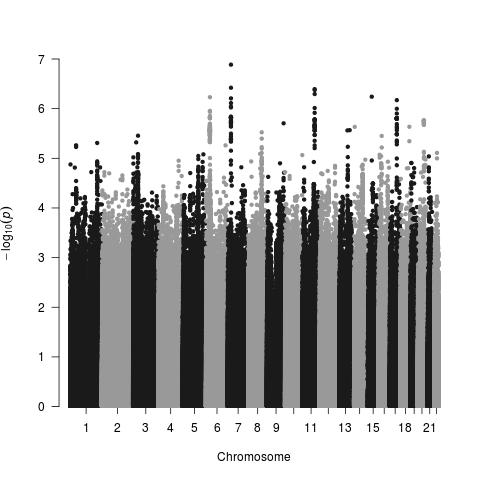
\includegraphics[width=0.8\linewidth]{{ukb_assoc/figure/manhatten_plots/manhatten_plot_4526}.jpeg}
    \caption{Manhattan plot for Impulsive aggression}\label{fig:ImpAgmanhatten}
  \end{subfigure}
  \caption{Manhattan and QQ Plot for Impulsive aggression.
    No genome wide significant SNPs was identified.\label{fig:gwas_impAgg}}
\end{figure}

\begin{table}[!htpb]
	\centering
	%latex.default(out, file = paste0(outputfolder, "ldscore_results_",     variable_name, ".tex"), table.env = F, rowname = NULL)%
\begin{center}
\begin{tabular}{llll}
\hline\hline
\multicolumn{1}{c}{Total Observed scale h2}&\multicolumn{1}{c}{Lambda GC}&\multicolumn{1}{c}{Intercept}&\multicolumn{1}{c}{Ratio}\tabularnewline
\hline
0.0532 (0.012)&1.0496&1.0082 (0.0056)&0.1693 (0.1163)\tabularnewline
\hline
\end{tabular}\end{center}

  \caption{LDsc results for Impulsive aggression.
    The intercept and ratio indicate the degree of inflation caused by factors other than polygencity, such as polulation stratification.
    Standard errors are indicated in parenthesis.
  }\label{tab:LDscImpAgg}
\end{table}

To summaries, the here presented GWAS was unable to identfiy a genome wide significant SNP\@.
LD-score regression results did not suggest presents of population stratification and heritability was estiamted at around 5\%.

\subsection{Risk Taking}
\label{sub:risk_taking_gwas}

In contrast to impulsive aggression, risk taking has a considerable sample size.
In total there were $120,286$ subjects available with a complete phenotype.
The corresponding QQ and Manhattan plot are displayed in figure~\ref{fig:risktaking_gwas}, and the lead SNPs are shown in table~\ref{tab:lead_snps_risk}.
As mentioned above, lead SNPs were identified using clumping.
LD-score regression indicates no major population stratification since both intercept and ratio approaches $0$ (see table~\ref{tab:ldscrisk}).

\begin{table}[!htpb]
	\centering
	%latex.default(out, file = paste0(outputfolder, "ldscore_results_",     variable_name, ".tex"), table.env = F, rowname = NULL)%
\begin{center}
\begin{tabular}{llll}
\hline\hline
\multicolumn{1}{c}{Total Observed scale h2}&\multicolumn{1}{c}{Lambda GC}&\multicolumn{1}{c}{Intercept}&\multicolumn{1}{c}{Ratio}\tabularnewline
\hline
0.0552 (0.0052)&1.127&1.0056 (0.0069)&0.0422 (0.052)\tabularnewline
\hline
\end{tabular}\end{center}

  \caption{LDsc results for risk taking
    The intercept and ratio indicate the degree of inflation caused by factors other than polygencity, such as polulation stratification.
    Standard errors are indicated in parenthesis.
  }\label{tab:ldscrisk}
\end{table}


The Manhattan plot in figure~\ref{fig:riskmanhatten} shows two clear signal in chromosome 3 and 6, as well as a signal which is just below genome wide significant at chromosome 4.
A closer inspection of the signal in chromosome 3 shows 2 lead SNPs (see table~\ref{tab:lead_snps_risk}).

\begin{figure}[!htpb]
	\begin{subfigure}{.5\textwidth}
		\centering
		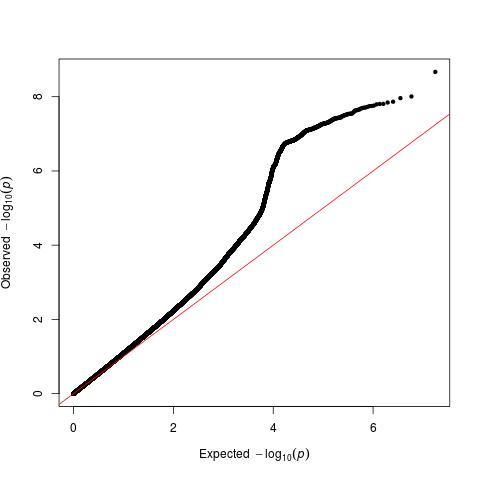
\includegraphics[width=0.8\linewidth]{{ukb_assoc/figure/qq_plots/qq_plot_2040}.jpeg}
		\caption{QQ-Plot of risk taking}\label{fig:riskqq}
	\end{subfigure}
	\begin{subfigure}{.5\textwidth}
		\centering
		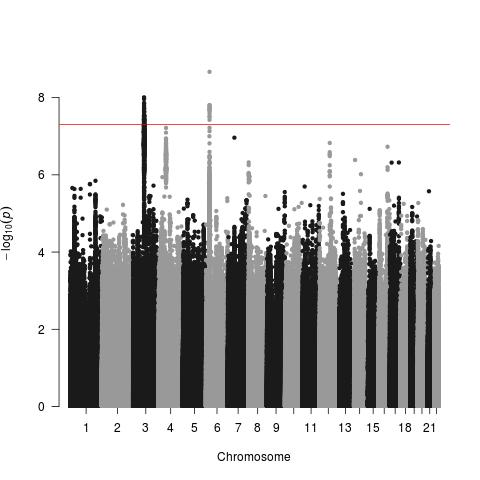
\includegraphics[width=0.8\linewidth]{{ukb_assoc/figure/manhatten_plots/manhatten_plot_2040}.jpeg}
		\caption{Manhattan plot of risk taking}\label{fig:riskmanhatten}
	\end{subfigure}
  \caption{GWAS on Risk Taking\label{fig:risktaking_gwas}}
\end{figure}

\begin{table}
	\small
	\centering
	%latex.default(dat, title = "", file = paste0(outputfolder, "lead_snp_",     nameID, ".tex"), digits = 3, rowname = NULL, table.env = F)%
\begin{tabular}{rlrlrrrr}
\hline\hline
\multicolumn{1}{c}{CHR}&\multicolumn{1}{c}{SNP}&\multicolumn{1}{c}{BP}&\multicolumn{1}{c}{A1}&\multicolumn{1}{c}{N}&\multicolumn{1}{c}{OR}&\multicolumn{1}{c}{STAT}&\multicolumn{1}{c}{P}\tabularnewline
\hline
$3$ & rs13084531 & $85553994$ & G & $115264$ & $0.936$ & $5.73$ & $9.83e-09$\tabularnewline
$6$ & rs9379971  & $27259308$ & T & $109344$ & $1.065$ & $ 5.99$ & $2.14e-09$\tabularnewline
\hline
\end{tabular}

	\caption{Lead SNPs reaching genome wide significance in Risk Taking}\label{tab:lead_snps_risk}
\end{table}

However, \textit{rs1308431} and \textit{rs7639518} have opposite directions of effect.
In order to investigate if the signals are independent of each other I performed a conditional analysis.
Using the top SNP (\textit{rs13084531}) as a covariate, the analysis showed no independent genome-wide significant effect.
Thus suggesting that \textit{rs7639518} is not independent of \textit{rs13084531}.
However, a closer look at the conditional regression model suggest that the \textit{rs7639518} might be a potentially independent signal (see table~\ref{tab:conditional}) since the resulting p-value is relatively low. 

\begin{table}[!htpb]
	\small
	\centering
	\resizebox{\textwidth}{!}{%latex.default(dat, title = "", file = "conditional_analysis_rs13084531.tex",     table.env = F, col.names = F)%
\begin{tabular}{lrlrlrrrr}
\hline\hline
\multicolumn{1}{l}{}&\multicolumn{1}{c}{CHR}&\multicolumn{1}{c}{SNP}&\multicolumn{1}{c}{BP}&\multicolumn{1}{c}{A1}&\multicolumn{1}{c}{NMISS}&\multicolumn{1}{c}{OR}&\multicolumn{1}{c}{STAT}&\multicolumn{1}{c}{P}\tabularnewline
\hline
2&$3$&rs76395182&$85547337$&G&$107738$&$0.957$&$-3.787$&$0.0001523$\tabularnewline
\hline
\end{tabular}
}
	\caption{Risk Taking with \textit{rs13084531} as covariate for selected SNP}\label{tab:conditional}
\end{table}

Below I will describe the three identified regions of interest (the two genome wide significant signals as well as the one approaching significance).
I also performed a quick literature review as well as looked up the three SNPs in the GWAS catalog (see table~\ref{tab:gwas_risk_catalog})

\paragraph{rs9379971}
\label{par:rs9379971}
This particular variant has the strongest association among all tested SNPs with a p-value of $2.14e-09$. 
The SNP is an intronic variant, without any mentioning in the GWAS catalog~\cite{Welter2014}.
As you can see in the LocusZoom plot (figure~\ref{fig:rs9379971}) the region round the identified SNPs is rather dense. 
The SNPs has been associated with \textit{POM121L2} and the region has been connected with schizophrenia across multiple studies~\cite{Aberg2013,Shi2009}.
However, the function of \textit{POM121L2} is not well understood.

\paragraph{rs13084531}
\label{par:rs13084531}
As you can see in figure~\ref{fig:rs13084531} the variant is in a relatively large LD region with a comparable p-value to the previous SNP ($9.826e-09$).
The SNPs is an intron variant within the gene \textit{CADM2}.
The gene has been associated with BMI~\cite{Speliotes2010} as well as executive functions and processing speed~\cite{Ibrahim-Verbaas2015}.
Interestingly the SNP associated in the study by~\cite{Ibrahim-Verbaas2015} (rs17518584) is in LD to our loci (rs13084531 with $R^2=0.4951;D'=0.9983$).
Hence suggesting a common loci for executive functions and risk taking.
Further the region of this SNP (3p12.1) has been connected to spirometric measures in smokers~\cite{Lutz2015}.

\paragraph{rs4386663}
\label{par:rs4386663}
This SNP is an intergenic variant with no known association with any regulatory functions.
However, the SNP is only marginal significant ($6.059e-08$).
Interestingly, however, the chromosomal region of this SNP (chr4q12) was also associated with spirometric measures in smokers by the same study as in variant rs13084531 (see paragraph~\ref{par:rs13084531}).
The LocusZoom plot (see figure~\ref{fig:rs13084531}) suggests a relatively narrow LD region. 

\begin{table}[!htpb]
	\centering
	\resizebox{\textwidth}{!}{%latex.default(dat, title = "", file = paste0(outputfolder, "gwas_catalog_",     nameID, ".tex"), digits = 3, rowname = NULL, table.env = F)%
\begin{tabular}{lrlrlrl}
\hline\hline
\multicolumn{1}{c}{Lead SNP}&\multicolumn{1}{c}{P}&\multicolumn{1}{c}{Study SNP}&\multicolumn{1}{c}{Study P}&\multicolumn{1}{c}{Disease Trait}&\multicolumn{1}{c}{PubMedID}&\multicolumn{1}{c}{Direction}\tabularnewline
\hline
rs13084531&$9.83e-09$&rs9841144&$9e-07$&Longevity (90 years and older)&$25199915$&yes\tabularnewline
rs13084531&$9.83e-09$&rs13323436&$3e-06$&Visceral fat&$22589738$&\tabularnewline
rs9379971&$2.14e-09$&rs16897515&$4e-07$&Schizophrenia&$23894747$&no\tabularnewline
rs9379971&$2.14e-09$&rs6932590&$1e-12$&Schizophrenia&$19571808$&yes\tabularnewline
\hline
\end{tabular}
}
	\caption{Additional SNP catalog look up for Risk Taking}\label{tab:gwas_risk_catalog}
\end{table}

\subsection{Conditional FDR}
\label{sub:conditional_fdr}

Figure~\ref{fig:cFDR} shows the conditional QQ plots for both aggression and risk taking for each of the chosen thresholds.
Both aggression and risk taking, conditional on each other did not result in any noticiable pleiotropic effect.
However, while aggression conditional on neuroticisim did not result in an inflation within the conditional QQ plots, risk taking was noticiable inflated conditional on SNPs which reached a relatively low p-value cutt-off.
Thus indicating considerable pleiotropic effects between risk taking and neuroticisim.
Further, these effects seem to particular be present at SNPs bellow $p\leq0.1$, but not at lower thresholds thus suggesting it is unlikely that both phenotypes share a common biological pathway.

\begin{figure}[!htpb]
  \centering
	\begin{subfigure}{0.4\textwidth}
		\centering
		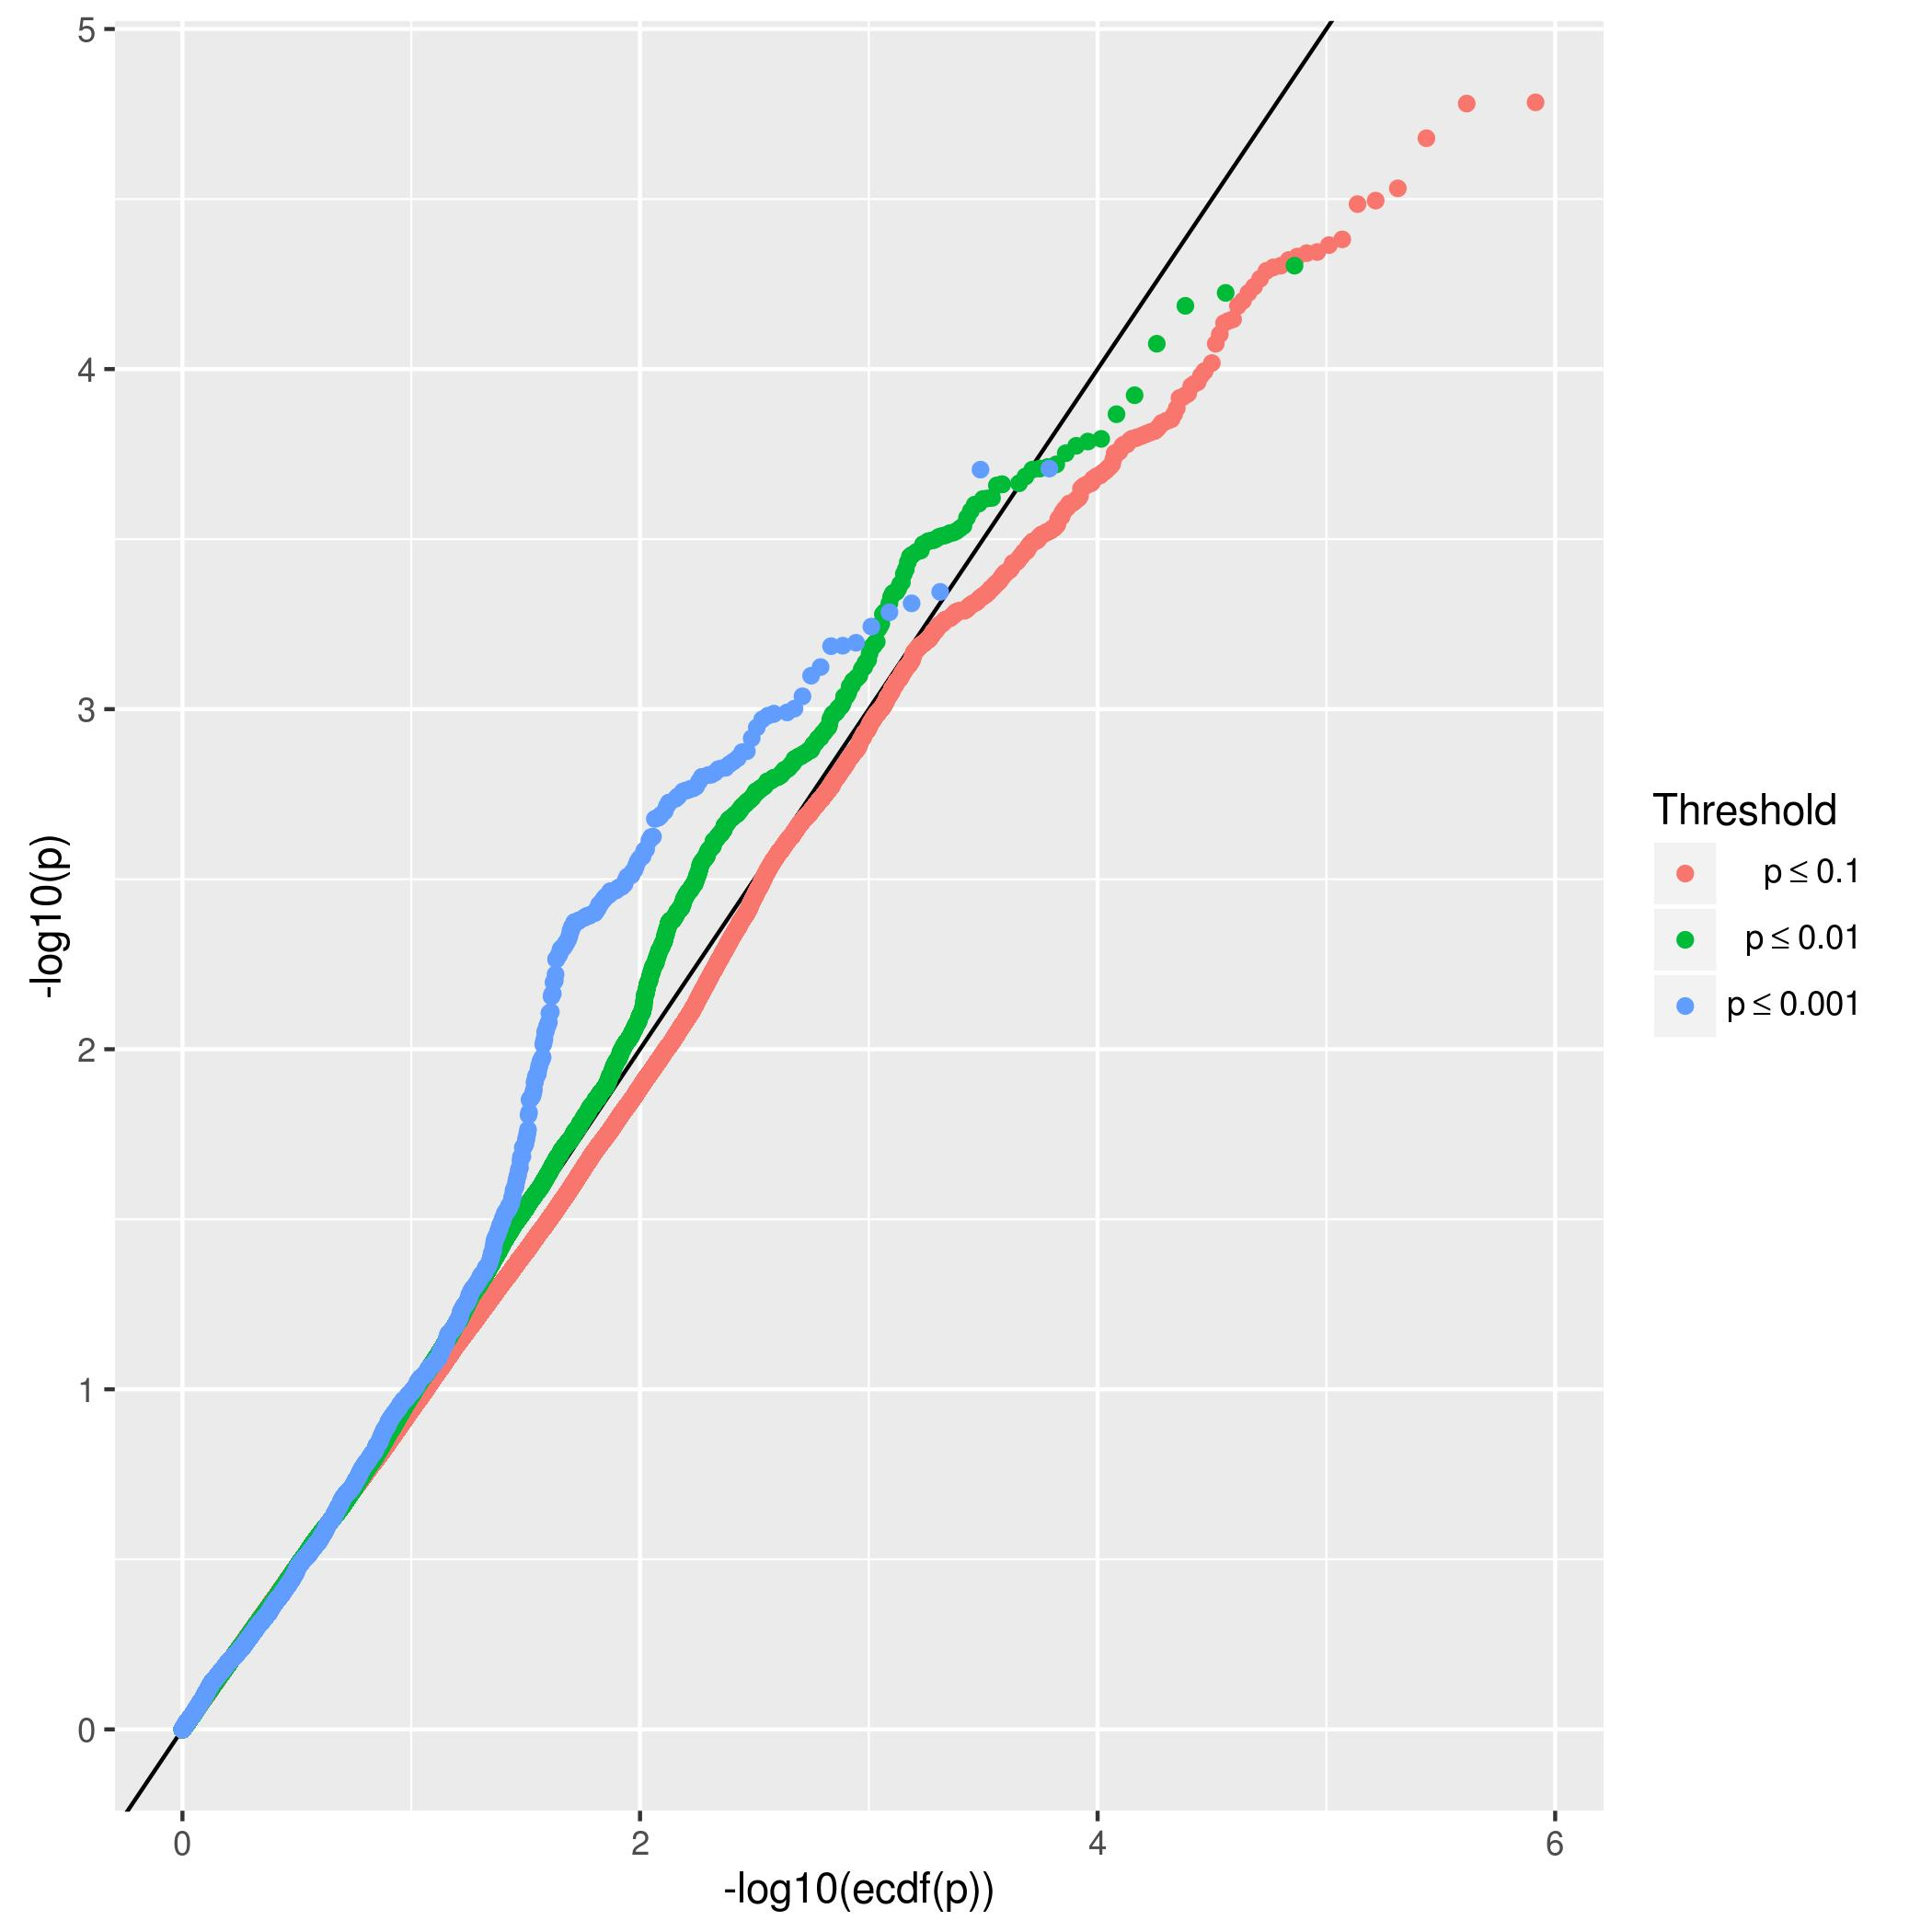
\includegraphics[width=0.9\linewidth]{ukb_assoc/figure/cFDR/risk.jpeg}
		\caption{QQ plot for risk taking, conditional on impulsive aggression\label{fig:cFDR_risk}}
	\end{subfigure}
	\begin{subfigure}{0.4\textwidth}
		\centering
		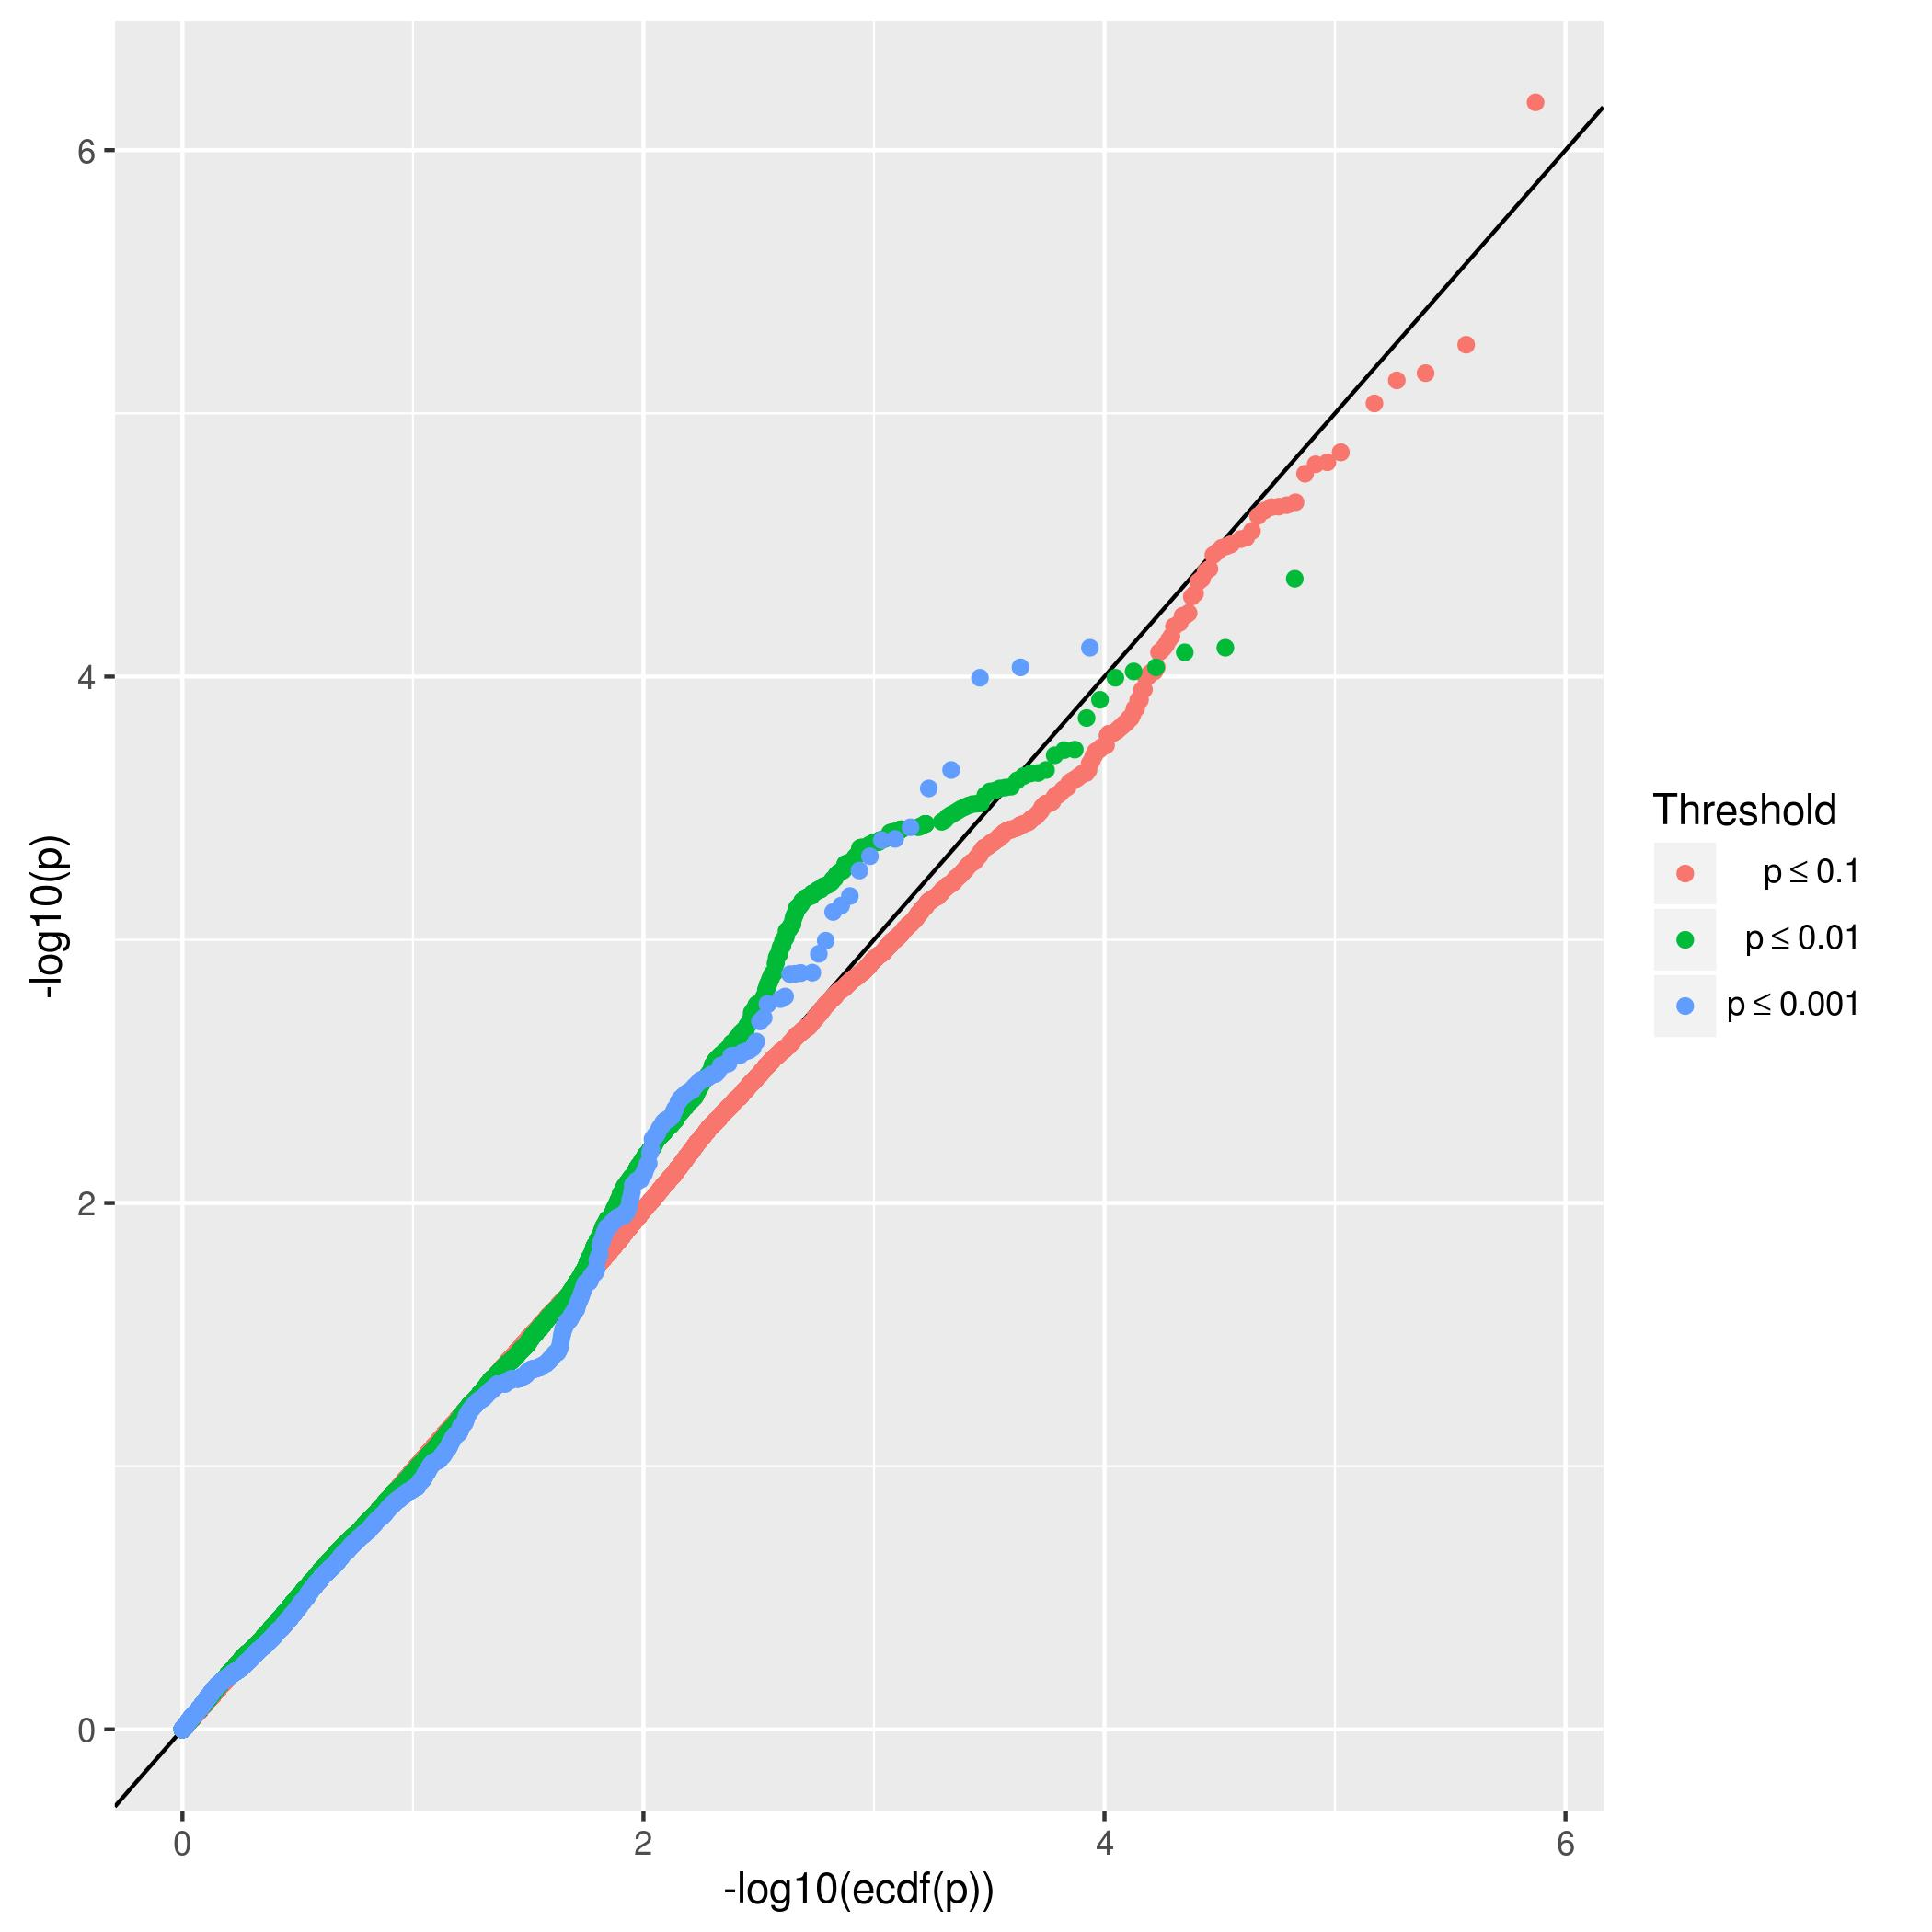
\includegraphics[width=0.9\linewidth]{ukb_assoc/figure/cFDR/aggresion.jpeg}
		\caption{QQ plot for impulsive aggression, conditional on risk taking\label{fig:cFDR_agg}}
	\end{subfigure}
	\begin{subfigure}{0.4\textwidth}
		\centering
    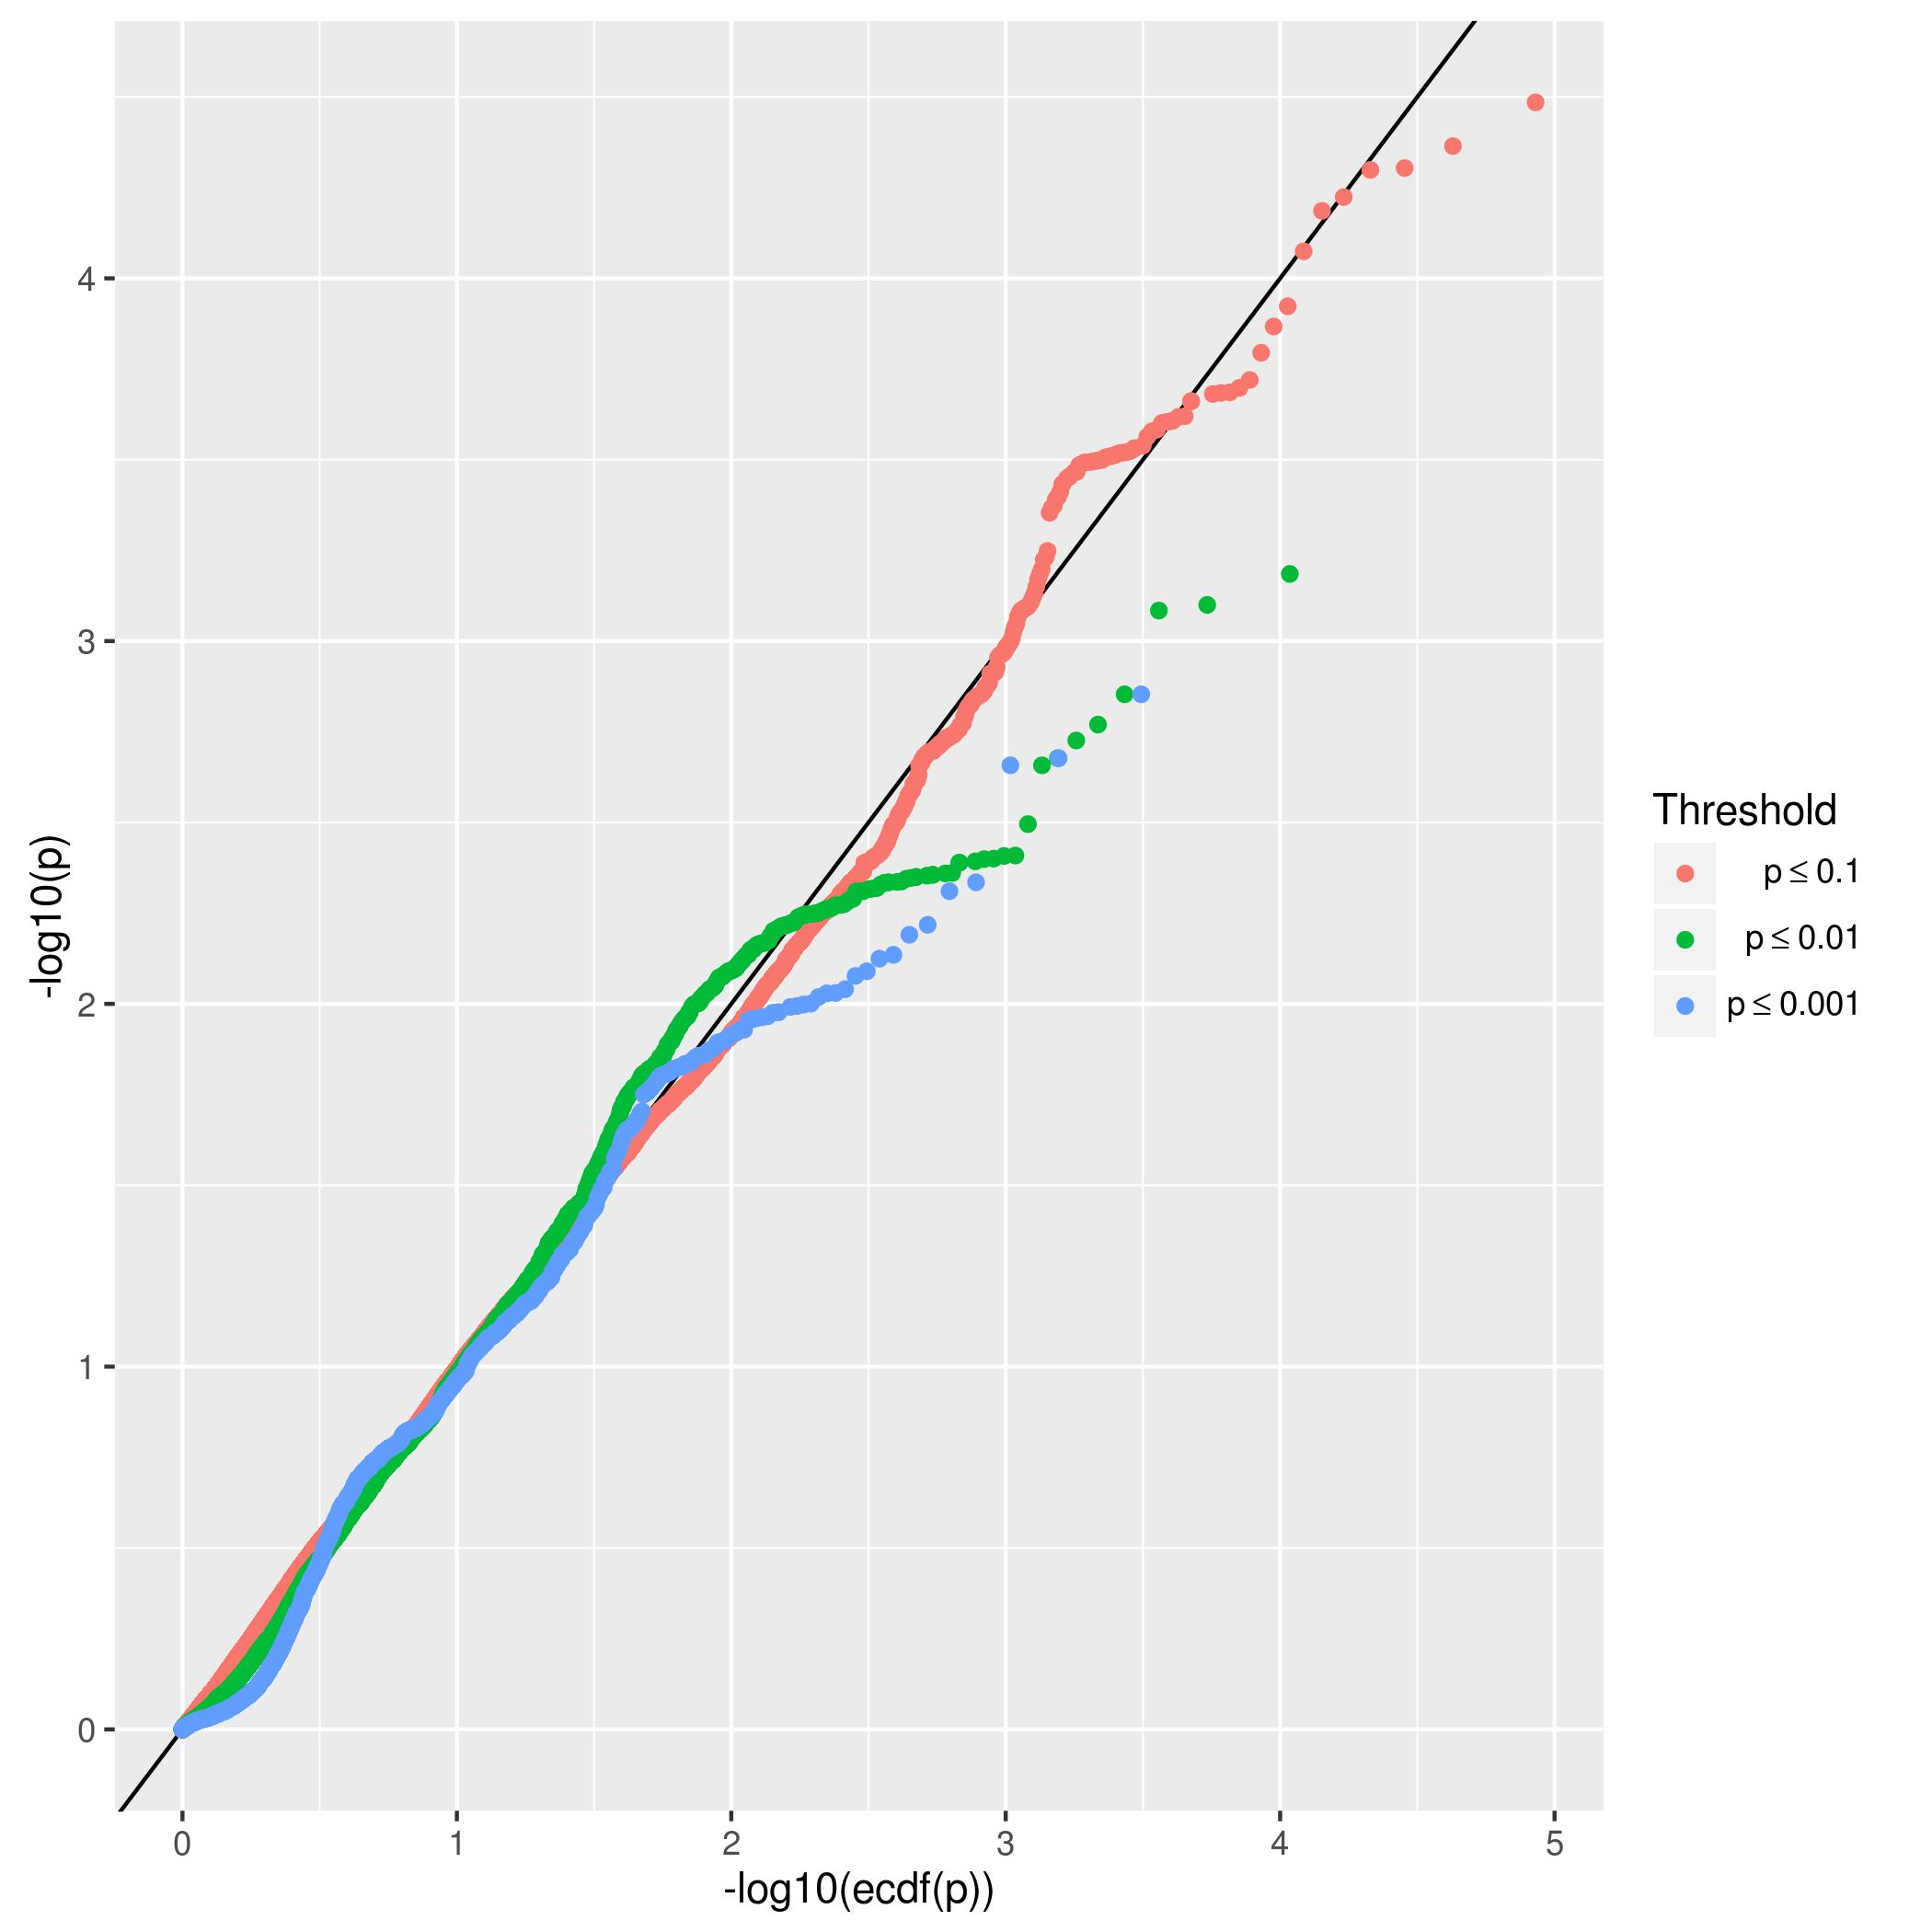
\includegraphics[width=0.9\linewidth]{ukb_assoc/figure/cFDR/aggresion_neuro.jpeg}
    \caption{QQ plot for impulsive aggression, conditional on neuroticisim\label{fig:cFDR_agg+neuro}}
	\end{subfigure}
	\begin{subfigure}{0.4\textwidth}
		\centering
    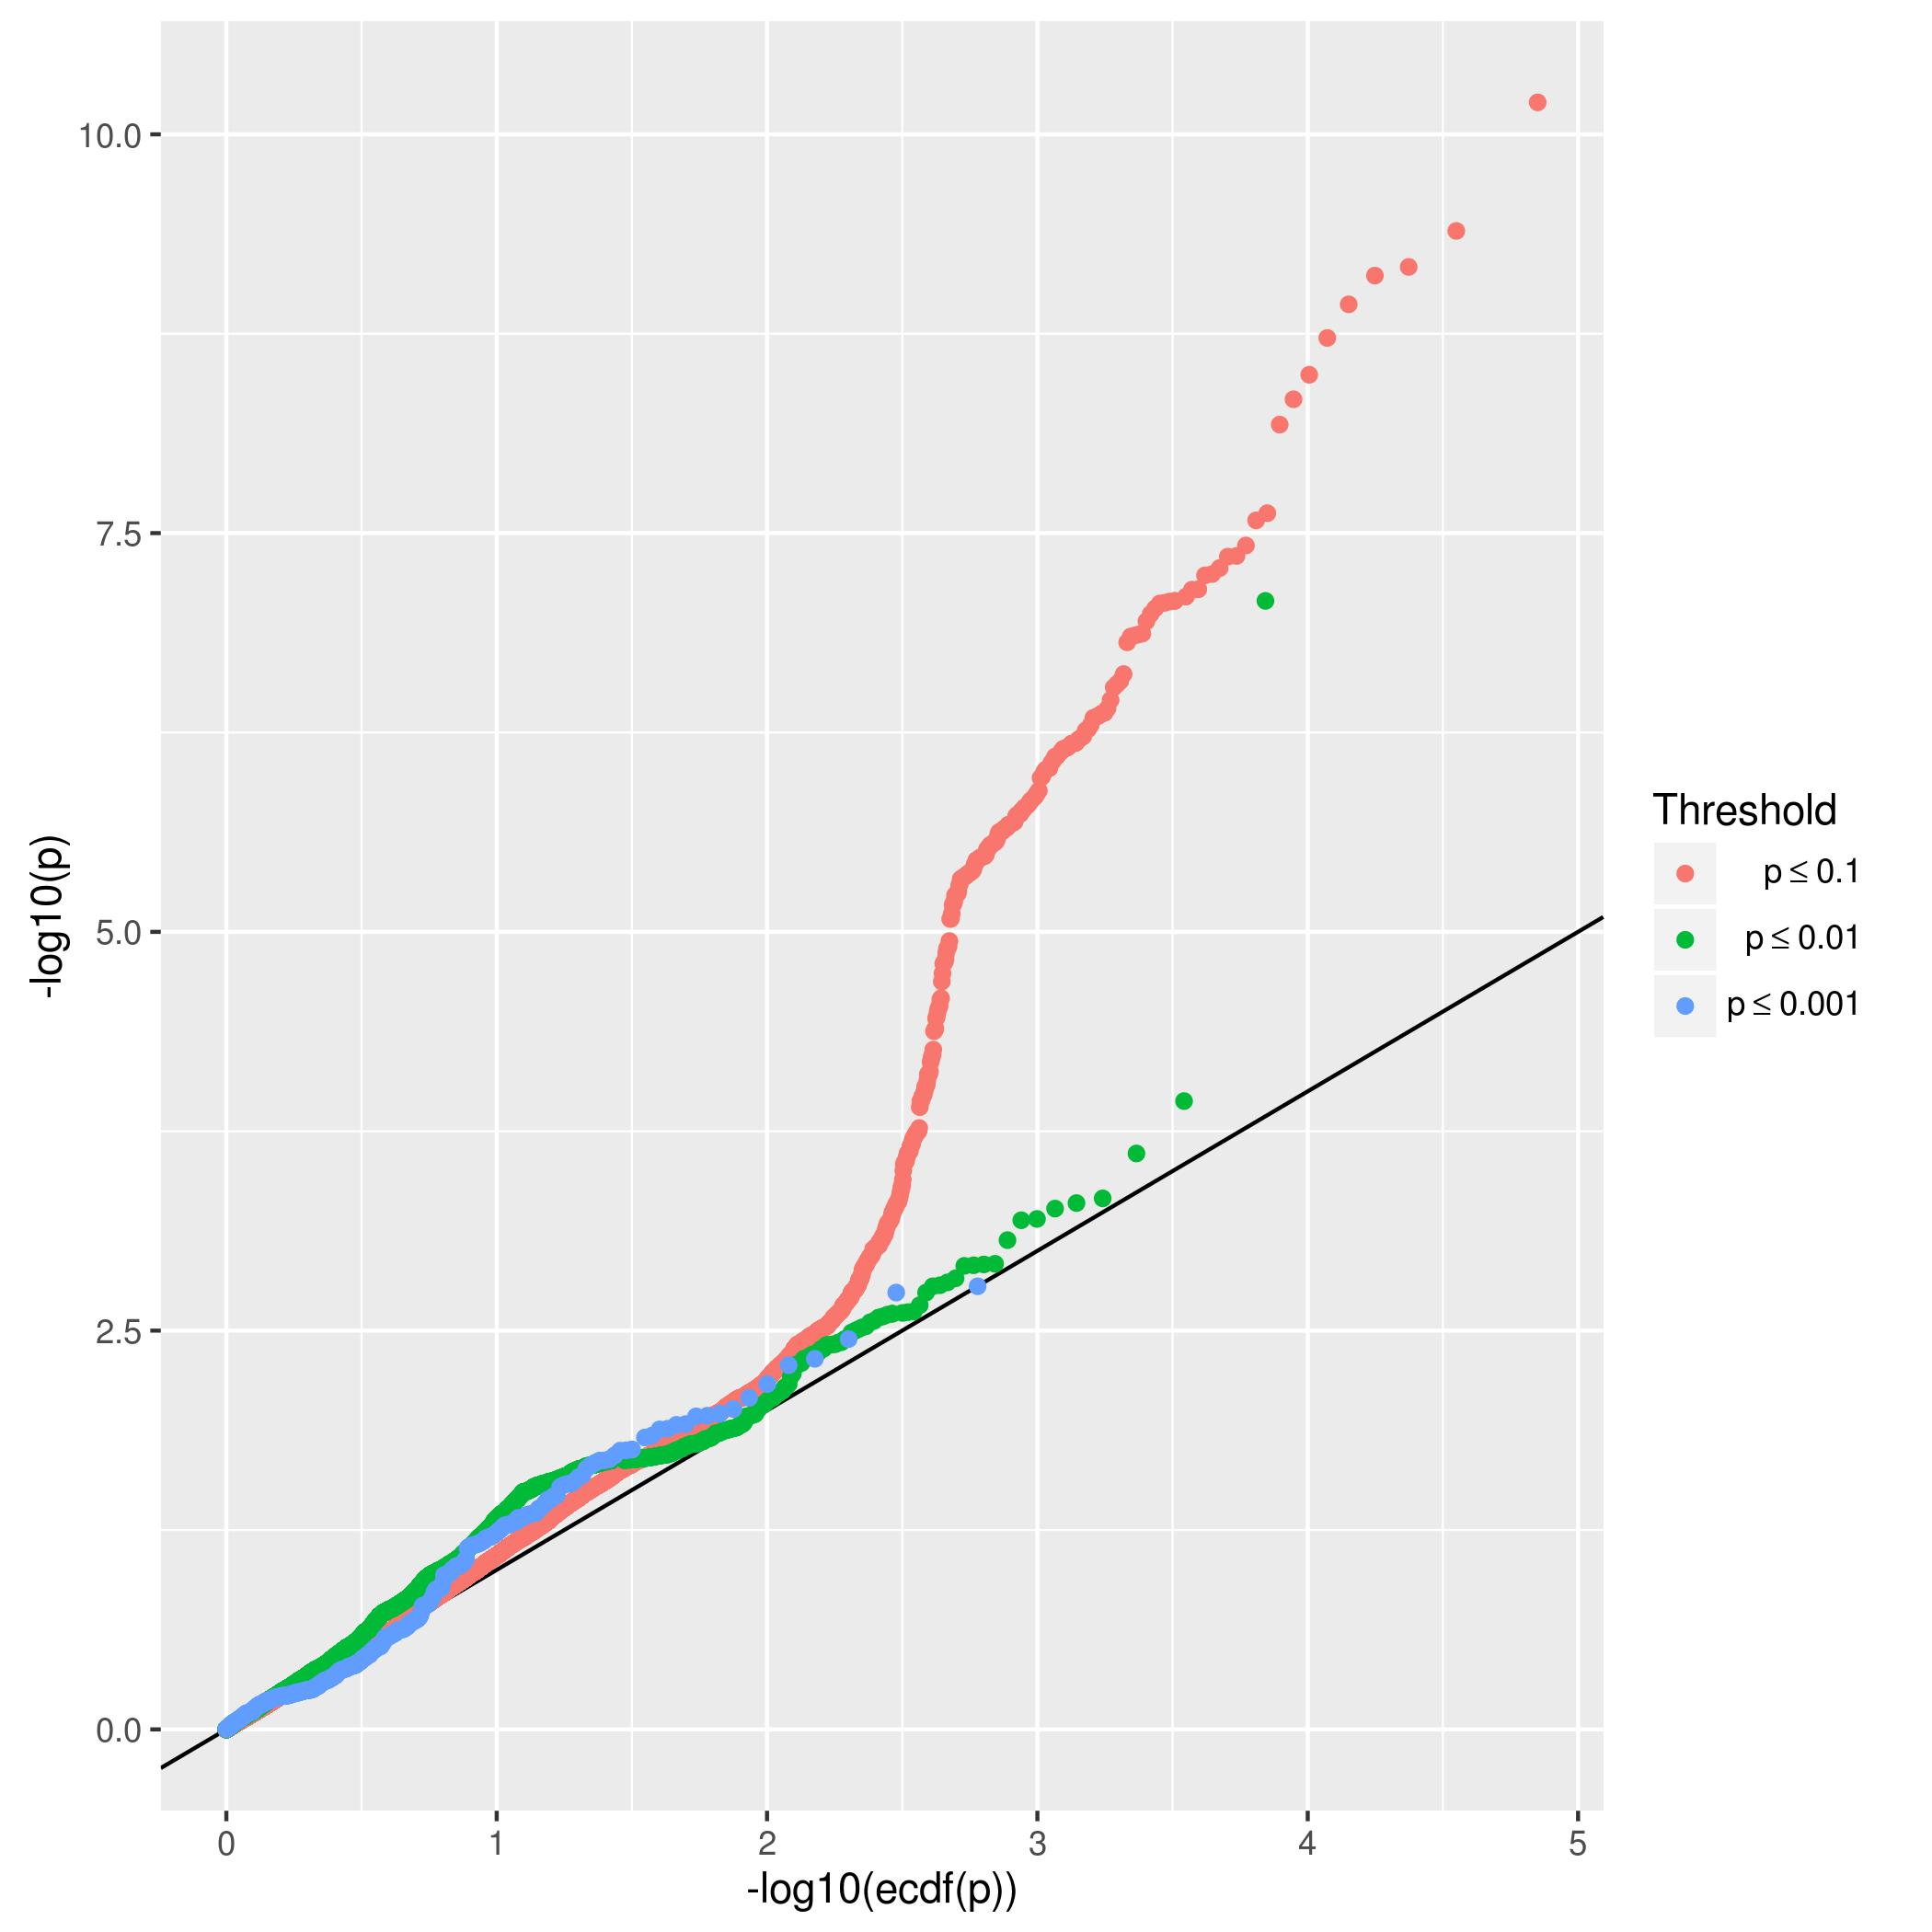
\includegraphics[width=0.9\linewidth]{ukb_assoc/figure/cFDR/risk_neuro.jpeg}
		\caption{QQ plot for impulsive aggression, conditional on neuroticisim\label{fig:cFDR_agg+neuro}}
	\end{subfigure}
  \caption{Conditional QQ plots for both risk taking and aggression, conditional on each other as well as neuroticisim.\label{fig:cFDR}}
\end{figure}

\subsection{Genetic Correlations}
\label{sub:genetic_correlations_internal}

Figure~\ref{fig:gcor} displays the genetic correlations of which all are significant at $\alpha=0.05$.

\begin{figure}[!h]
	\begin{subfigure}{.5\textwidth}
	\centering
	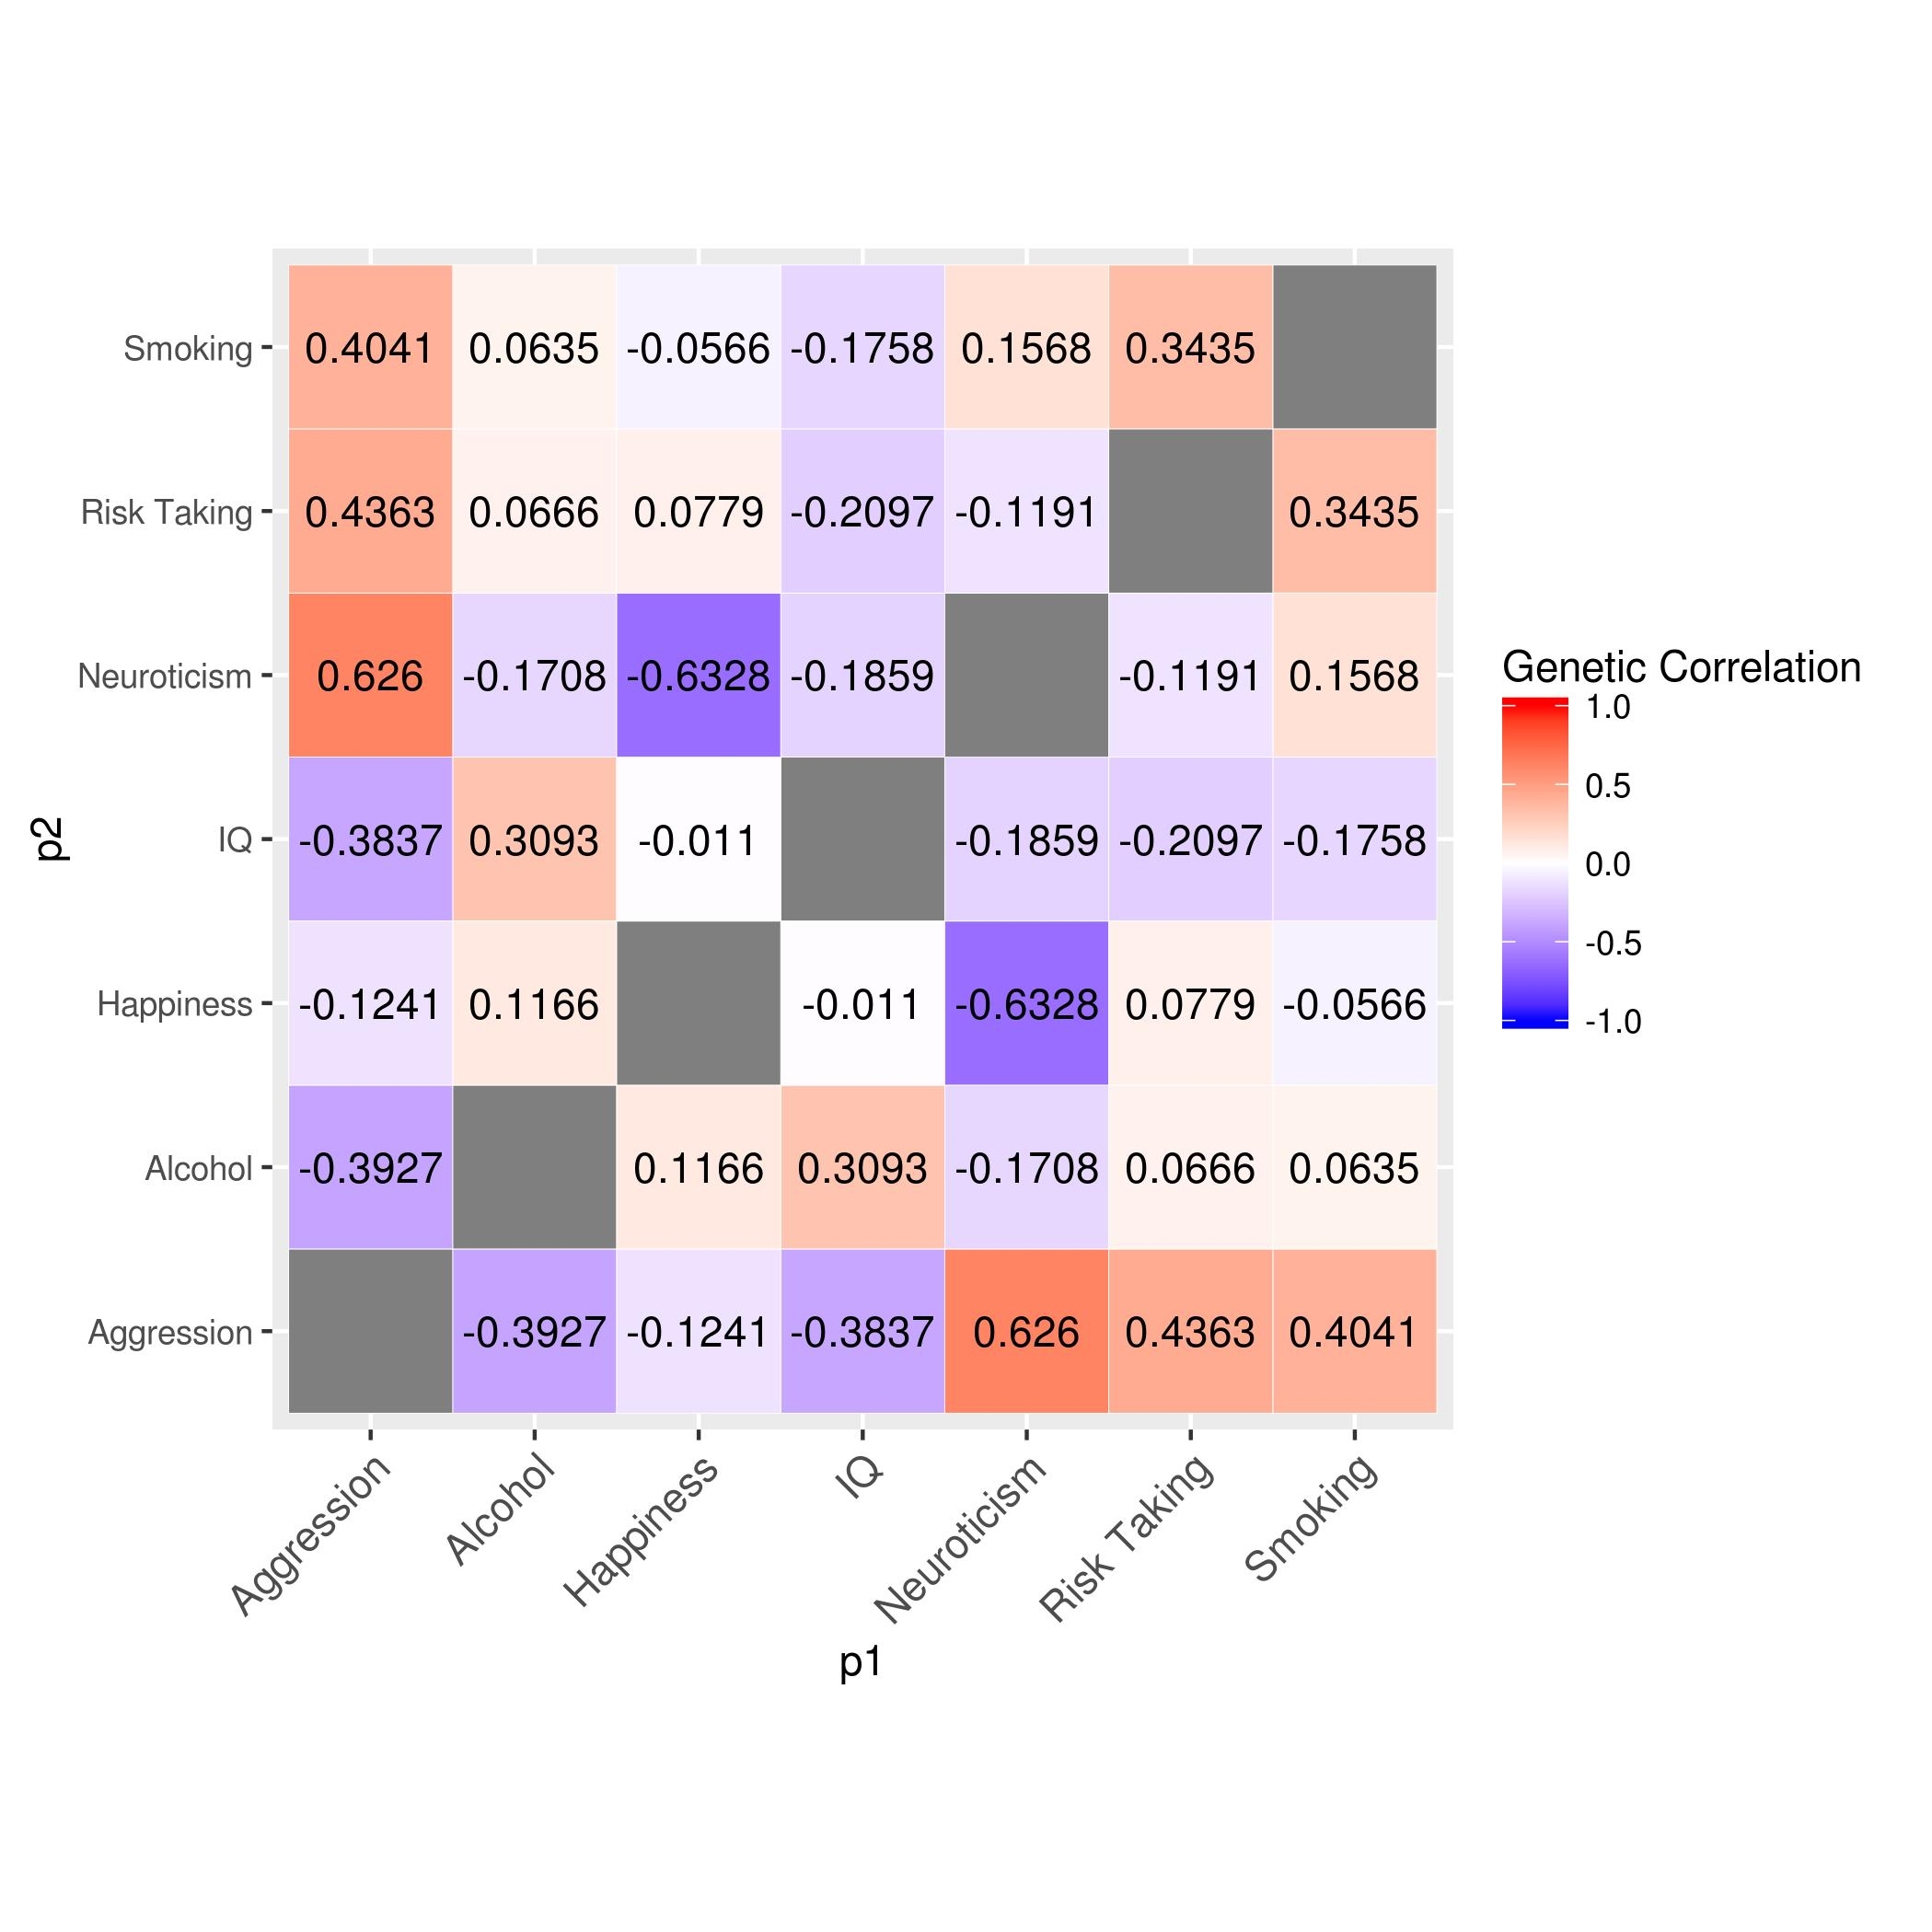
\includegraphics[width=1\linewidth]{{ukb_assoc/figure/genetic_corr/genetic_correlation_extended}.jpeg}
	\caption{Genetic Correlations}\label{fig:gcor}
	\end{subfigure}
	\begin{subfigure}{.5\textwidth}
	\centering
	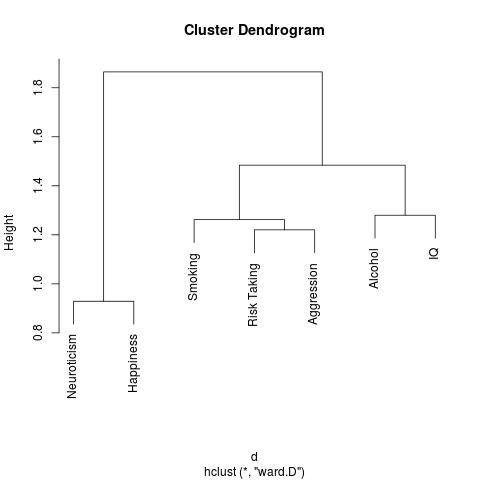
\includegraphics[width=1\linewidth]{ukb_assoc/figure/genetic_corr/dendrogram_correlations.jpeg}
	\caption{Hierarchical clustering of correlations}\label{fig:hirarCor}
	\end{subfigure}
\end{figure}

One can observe that, as one would expect, the genetic correlation between neuroticism and happiness is high ($-0.6328$) and both phenotypes cluster together.
A closer inspection of the correlation also shows that the estimate is similar to the one found in the well-being GWAS\@.

Additional one can observe a second cluster containing two sub-clusters.
These two correlation cluster are risk taking, impulsive aggression and smoking as well as alcohol consumption and IQ\@.
It is interesting to see that we find considerable genetic correlation between risk taking and smoking ($0.3435$).
This is reflecting our finding in the previous section when we compared genome wide significant SNPs in risk taking to those found in the GWAS catalog.
These SNPs were also be found to be associated with spirometric measures in smokers.
This would suggest that the genetic architecture for risk raking is partially overlapping with that of smoking.
Further the genetic correlation between impulsive aggression and risk taking is considerable ($0.4363$).

Another point of interest is IQ\@.
While IQ has a positive correlation with alcohol consumption, it is negatively correlated with risk taking ($-0.2097$), smoking ($-0.1758$) and impulsive aggression ($-0.3837$).
Further there is no correlation between IQ and happiness but a moderate negative correlation with neuroticism ($-0.1859$).

While smoking has its strongest correlation with risk taking and impulsive aggression, happiness has its only correlation with notable effect size with neuroticism.
This would indicate that happiness is rather unrelated to the other phenotype. 
Neuroticism, on the other hand, is not only negatively correlated with happiness, but also with alcohol consumption ($0.1708$), IQ ($0.1859$), risk taking ($-0.1191$) and smoking ($0.1568$).
Furhter the large genetic correlation between impulsive aggression and neuroticism ($0.6260$) is of additional intersest.
